\chapter{Architektura}

\begin{figure}[ht]
  \centering
  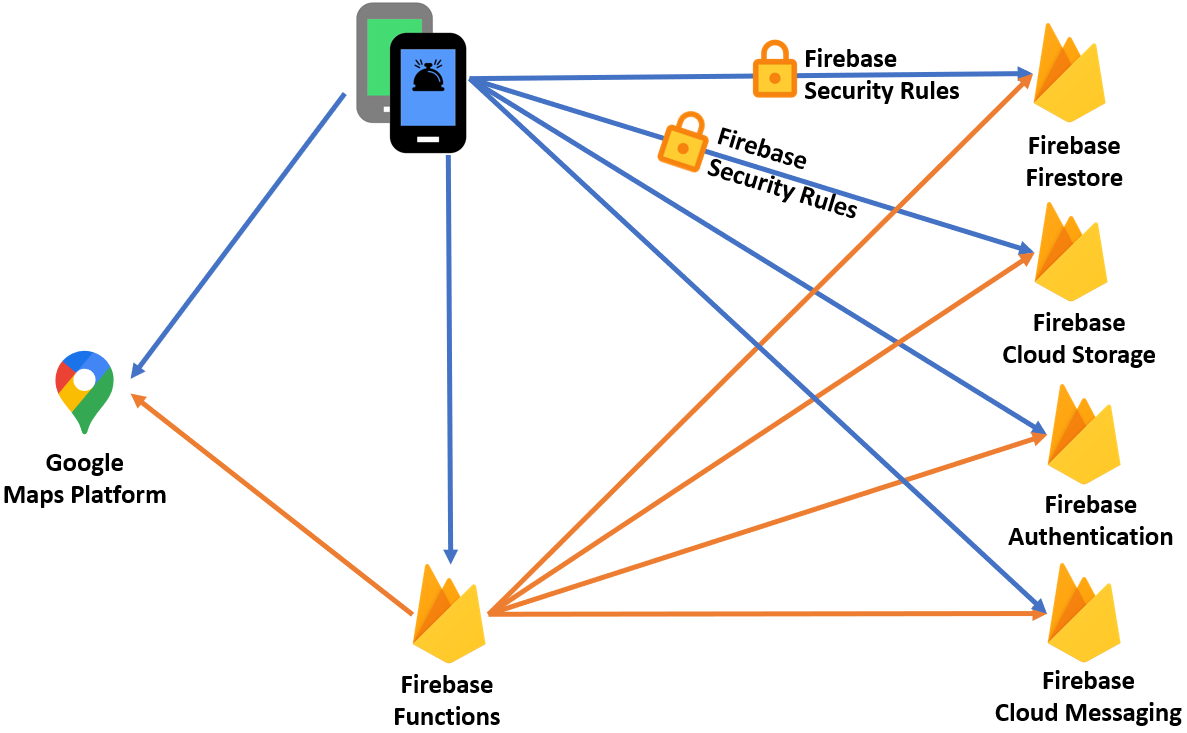
\includegraphics[width=\linewidth]{images/architecture.png}
  \caption{Schemat architektury systemu}
  \label{fig:architecture}
\end{figure}

Na rysunku \ref{fig:architecture} przedstawiona została wysokopoziomowa architektura stworzonego systemu. Składa się na nią siedem komponentów połączonych relacjami zależności.

Najważniejszym elementem z punktu widzenia użytkowników są aplikacje mobilne. W celu zapewnienia swojej funkcjonalności korzystają one ze wszystkich innych komponentów. Dostęp do bazy danych Firestore oraz magazynu plików Cloud Storage jest jednak ograniczony przez reguły bezpieczeństwa, by uniemożliwić wykonywanie przez użytkowników niepożądanych operacji.

Usługa Firebase Functions to drugi ważny komponent. Odgrywa rolę backendu. Aplikacje klienckie delegują do niej wykonywanie części operacji. Zajmuje się ona również synchronizacją pomiędzy różnymi częściami systemu. Jest to środowisko kontrolowane, więc żadne ograniczenia dostępu nie są potrzebne.

Implementacja przedstawionego systemu została podzielona na dwie równolegle rozwijane części. Pierwszą z nich stanowią aplikacje klienckie, a drugą projekt Firebase, który obejmuje funkcje Firebase Functions oraz reguły bezpieczeństwa Firebase Security Rules.

% Implementacja przedstawionego systemu została podzielona na dwie równolegle rozwijane części. Pierwszą z nich stanowią aplikacje klienckie, opisane w rozdziale \ref{part:applications}, a drugą projekt Firebase, przedstawiony w rozdziale \ref{part:firebase}. Włączają się w niego funkcje Firebase Functions oraz reguły Firebase security Rules. W osobnym rozdziale została opisana także baza danych, ponieważ obie części z niej korzystają.